\documentclass{article}
\usepackage[utf8]{inputenc}
\usepackage[margin=0.5in]{geometry}
\usepackage{tikz}
\usepackage{amsmath}
\usepackage{amssymb}

\begin{document}
\noindent
Dustin Newman

\noindent
CS 181, Discussion 1C

\noindent
Campbell, Mathur

{\centering
\Large{\textsc{Assignment Seven}}
\par}

\section{}
The DPDA for this language is $(\{q_0,A,B_1,E,B_2,C,q_A\}, \{a,b,c\}, \{\$,b\}, q_0, \{q_0,E,q_A\})$ where the transition function $\delta$ can be seen below:

\begin{center}
    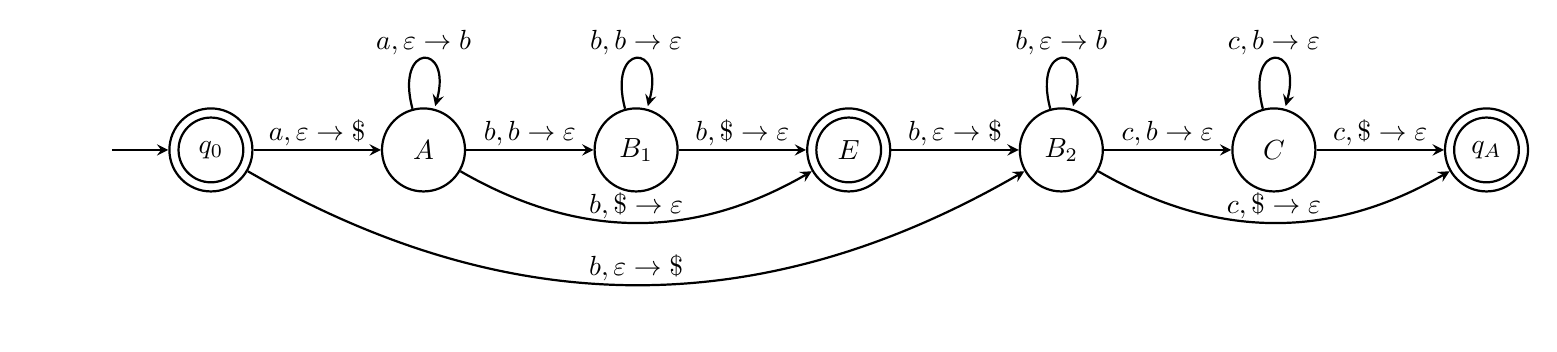
\begin{tikzpicture}[scale=0.9]
        \begin{scope}[auto, every node/.style={thick, draw, circle, minimum size=3em, inner sep = 1}]
            \node [draw=none] (I) at (-2,0) {};
            \node (q0) at (0,0) {\(q_0\)};
            \node (A) at (3,0) {\(A\)};
            \node (B1) at (6,0) {\(B_1\)};
            \node (E) at (9,0) {\(E\)};
            \node (B2) at (12,0) {\(B_2\)};
            \node (C) at (15,0) {\(C\)};
            \node (qa) at (18,0) {\(q_A\)};
            \draw[black, thick] (0,0) circle [radius=1.3em];
            \draw[black, thick] (9,0) circle [radius=1.3em];
            \draw[black, thick] (18,0) circle [radius=1.3em];
        \end{scope}
        \begin{scope}[auto, every node/.style={minimum size=1em,inner sep=1}, every path/.style={thick, ->, >=stealth}]
            \path (I) edge (q0);
            \path (q0) edge node {$a, \varepsilon \rightarrow \$$} (A);
            \path (A) edge [bend right] node {$b, \$ \rightarrow \varepsilon$} (E);
            \path (A) edge node {$b, b \rightarrow \varepsilon$} (B1);
            \path (B1) edge node {$b, \$ \rightarrow \varepsilon$} (E);
            \path (A) edge [loop above] node {$a, \varepsilon \rightarrow b$} (A);
            \path (E) edge node {$b, \varepsilon \rightarrow \$$} (B2);
            \path (B1) edge [loop above] node {$b, b \rightarrow \varepsilon$} (B1);
            \path (q0) edge [bend right] node {$b, \varepsilon \rightarrow \$$} (B2);
            \path (B2) edge [loop above] node {$b, \varepsilon \rightarrow b$} (B2);
            \path (B2) edge node {$c, b \rightarrow \varepsilon$} (C);
            \path (B2) edge [bend right] node {$c, \$ \rightarrow \varepsilon$} (qa);
            \path (C) edge [loop above] node {$c, b \rightarrow \varepsilon$} (C);
            \path (C) edge node {$c, \$ \rightarrow \varepsilon$} (qa);
        \end{scope}
    \end{tikzpicture}
\end{center}

\noindent
My DPDA works by recognizing that any string in the language can be partitioned into two substrings: one of $a^ib^i$ and one of $b^jc^j$. Then, $n = i + j$ becomes almost trivial to prove. We only need to handle the first substring if the input string begins with an $a$. If so, we transition to the DPDA that takes care of that, marking the first $a$ with a $\$$ from the stack alphabet. We only return from that machine if we have a valid $a^ib^i$ string to state $E$. Since $j = 0$ is allowed, we accept on $E$. If we see another $b$, we know we also have a $b^jc^j$ substring and so we handle that similarly in the second subset of the machine.

\newpage
\section{}

\begin{align*}
\underline{v} + v \times v + v &\rightarrowtail F + v \times v + v \\
\underline{F} + v \times v + v &\rightarrowtail T + v \times v + v \\
\underline{T} + v \times v + v &\rightarrowtail E + v \times v + v \\
E + \underline{v} \times v + v &\rightarrowtail E + F \times v + v \\
E + \underline{F} \times v + v &\rightarrowtail E + T \times v + v \\
E + T \times \underline{v} + v &\rightarrowtail E + T \times F + v \\
E + \underline{T \times F} + v &\rightarrowtail E + T + v \\
\underline{E + T} + v &\rightarrowtail E + v \\
E + v &\rightarrowtail E + F \\
E + \underline{F} &\rightarrowtail E + T \\
\underline{E + T} &\rightarrowtail E
\end{align*}

\newpage
\section{}
\subsection{}
\begin{align*}
\underline{()}()()() &\rightarrowtail S()()() \\
S\underline{()}()() &\rightarrowtail SS()() \\
\underline{SS}()() &\rightarrowtail S()() \\
S\underline{()}() &\rightarrowtail SS() \\
SS\underline{()} &\rightarrowtail SSS \\
S\underline{SS} &\rightarrowtail SS \\
\underline{SS} &\rightarrowtail S
\end{align*}

\subsection{}
\begin{align*}
\underline{()}()()() &\rightarrowtail S()()() \\
S\underline{()}()() &\rightarrowtail SS()() \\
SS\underline{()}() &\rightarrowtail SSS() \\
SSS\underline{()} &\rightarrowtail SSSS \\
SS\underline{SS} &\rightarrowtail SSS \\
S\underline{SS} &\rightarrowtail SS \\
\underline{SS} &\rightarrowtail S
\end{align*}

\end{document}
